\documentclass[12pt, oneside]{article}
\usepackage[letterpaper]{geometry}
\usepackage{Logemann}
\usepackage{SetTheory}
\usepackage{Sum}
\usepackage{Product}
\usepackage{listings}
\usepackage{jlcode}

\begin{document}
\noindent \textbf{\Large{Caleb Logemann \\
AERE 504 Intelligent Air Systems \\
Project 1
}}

\section{Description of Methods}
  For this project I implemented both the k2 search algorithm and the local
  search algorithm.
  The k2 algorithm starts with a ordering of the variables and then generates
  a Bayesian Network structure that maximizes the Bayesian score and such that
  the ordering is a topological sort of the nodes.
  The local search algorithm starts from a random structure and then takes
  local moves to maximize the Bayesian score.

  For my full search algorithm I used a combination of both of these algorithms.
  I first generated a random ordering of variables and then applied the k2 algorithm.
  I then used the local search on the result of the k2 search.
  This can only improve upon the result of the k2 algorithm and guarantees that
  I am at a local maximum.
  I also used a randomized restarting process to more fully search the space
  and to make sure the algorithm didn't get stuck at a poor local maximum.

  Overall this could be viewed in two different perspectives, the first is that
  I am running a randomized restart of the local search algorithm, where the k2
  algorithm is generating the random initial structure.
  The second perspective is that I am running a randomized restart on the k2
  algorithm and then post processing with the local search to further optimize
  the solution.
  I think the second perspective may be more appropriate as I believe the k2
  algorithm to be doing most of the optimizing.
\section{Graphs and Scores}
  \begin{center}
    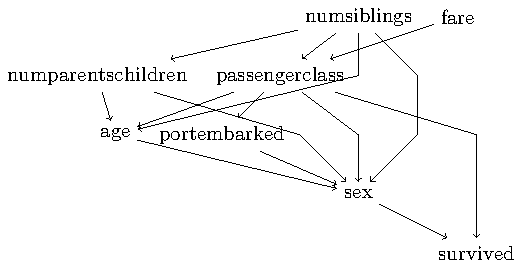
\includegraphics[scale=0.8]{titanic.pdf}
  \end{center}
  The Bayesian Score for this structure is -3794.8556
  It took 58.37 seconds to compute a 1000 random restarts.
  Some interesting interpretations can be seen in this graph structed.
  For example if a passenger survived depending mostly on the sex of the
  passenger and class of the passenger.
  Also a passenger's class, fare, and age are related as well as the number
  of siblings and the number of parents children.
  \begin{center}
    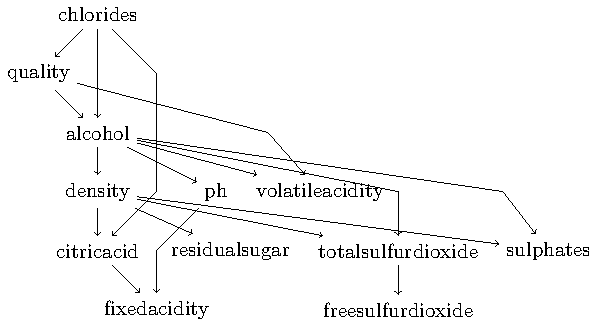
\includegraphics[scale=0.8]{whitewine.pdf}
  \end{center}
  The Bayesian Score for this structure is -41958.9109.
  It took 968.50 seconds to compute a 1000 random restarts.
  Interpreting this graph, we see that the quality of the wine mainly depends
  on the alcohol and the volatile acidity of the wine.
  The density of the wine is related to the sugars, alcohol, citric acid,
  sulphates, and totalsulfurdioxide.
  There are also several other relationships between closely related aspects of
  the wine.
  \begin{center}
    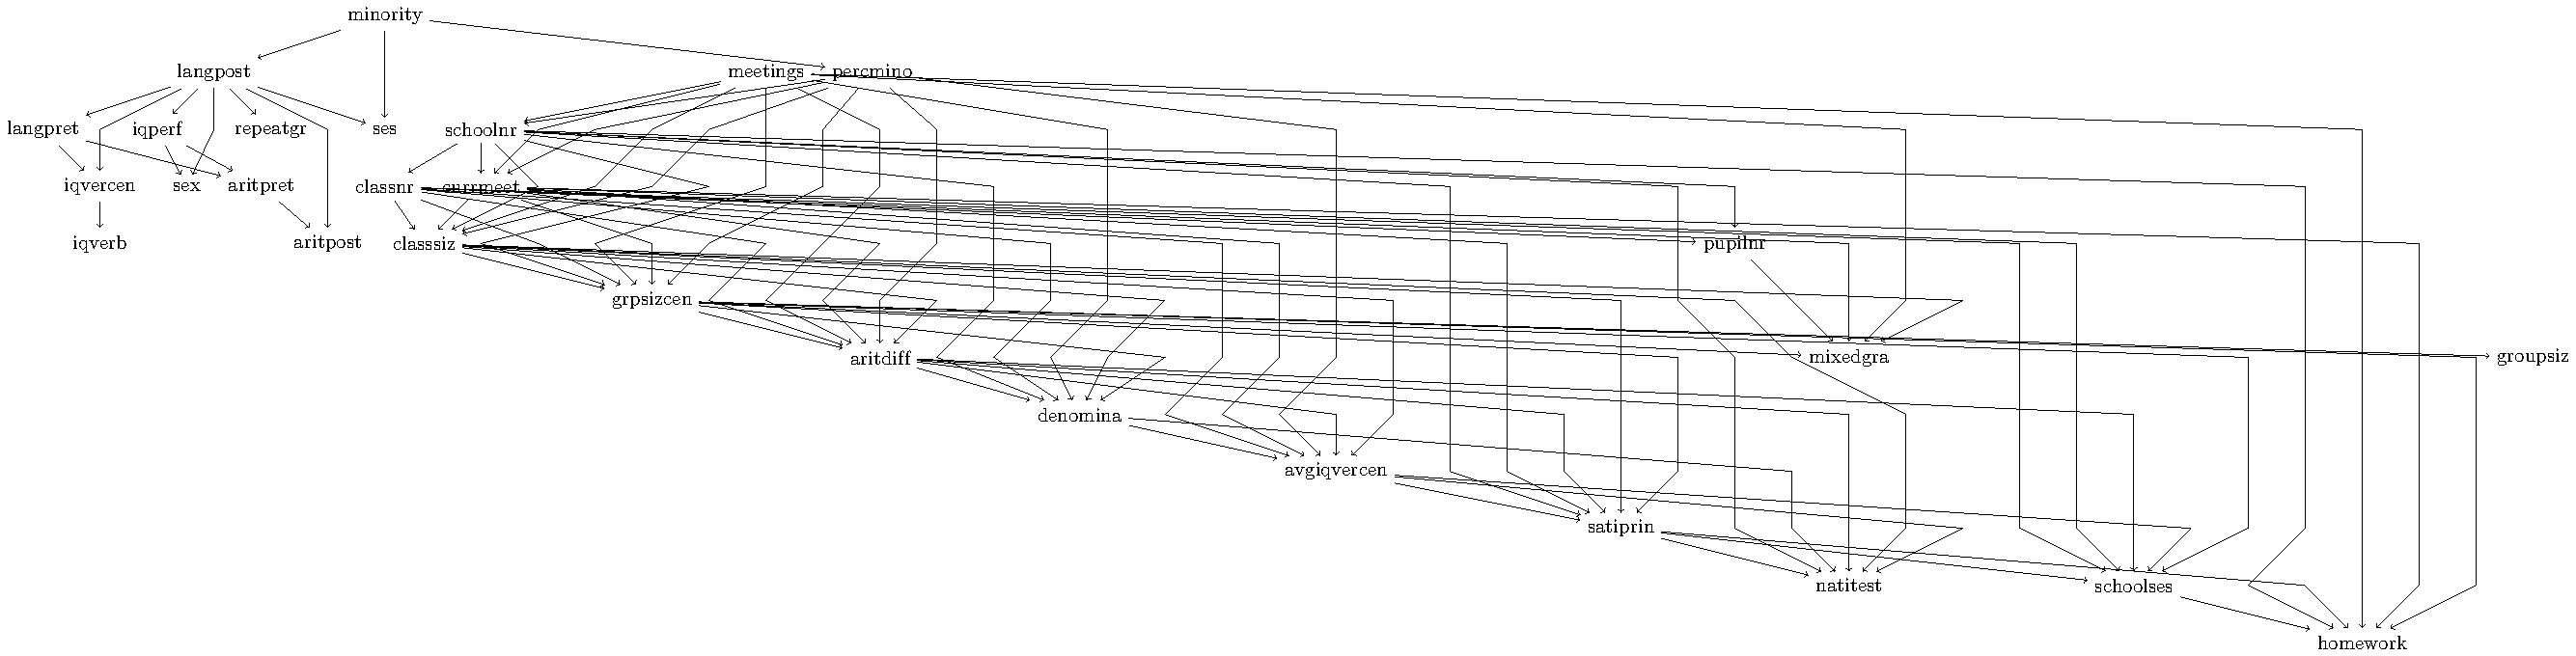
\includegraphics[scale=0.35]{schoolgrades.pdf}
  \end{center}
  The Bayesian Score for this structure is -43302.7933.
  It took 8474.55 seconds to compute 500 random restarts.
  Interpreting this graph is rather difficult, and the relationships between
  different variables is convoluted.
  One key relationship is that between minority status and socio-economic status.
  Also currmeet, classsiz, and grpsizcen all seem important as they have a lot of
  parents and a lot of children.
  \begin{center}
    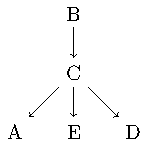
\includegraphics[scale=0.5]{structurelearning_test.pdf}
  \end{center}
  The Bayesian Score for this structure is -2211.0642.
  It took 11.59 seconds to compute a 1000 random restarts.
  The main interpretation of this graph would be that all other variables are
  connected with variable C.

  \lstinputlisting[breaklines=true]{Project1.jl}
  \lstinputlisting[breaklines=true]{BayesianNetworks.jl}

\end{document}

